
\chapter{Introduction to binaries}

\section{Binary stars}

\subsection{What is a binary star ?}

When two massive bodies of mass $m_1$ and $m_2$ interact gravitationally, they can have different types of trajectory depending on their total energy:

\begin{equation}
E = E_k + E_p = \frac{1}{2} m_1 v_1^2 + \frac{1}{2} m_2 v_2^2  - \frac{G m_1 m_2}{\| \bold{r_1} - \bold{r_2}\| }.
\end{equation}

%\begin{itemize}
%\item[$\bold{E>0}$], the system is unbound, the bodies follow hyperbolic trajectories. They have a distance of closer approach then move away from each other forever.
%\item[$\bold{E=0}$], the system is marginally unbound, the bodies follow parabolic trajectories.
%\item[$\bold{E<0}$], the system is bound, the bodies have stable elliptical orbits around each others.
%\end{itemize}

If $E<0$, they are bound and locked in a binary system. Such systems are characterised by their semi-major axis $a$, their eccentricity $e$, their period $p$, their total mass $m_t = m_1 + m_2$, mass ratio $q = m_2/m_1$ with $m_1$ being the primary, more massive than $m_2$.
Mass, period and semi-major axis are related by Kepler's third law:

\begin{equation}
\frac{G m_t}{4\pi^2} =  \frac{a^3}{p^2}.
\end{equation}

Interestingly, expressed in AU, $\Mo$ and years, $G \simeq 4 \pi^2$, thus the law can be written:

\begin{equation}
\left( \frac{m_t}{1 \Mo} \right) \simeq \left( \frac{p}{1 \textrm{yr}} \right) \left( \frac{a}{1 \textrm{AU}} \right)^3 .
\end{equation}



\begin{figure}
\center
    \centering
    \begin{subfigure}[b]{0.48\textwidth}
    	\centering
        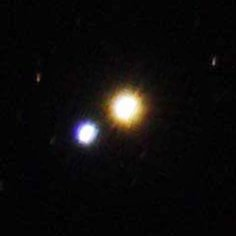
\includegraphics[width=0.6\textwidth]{Figures/0_albireo.jpg}
        \caption{Albireo ($\beta$ Cygni)}
        \label{Fig:0_binary_1}
    \end{subfigure}
    ~~
    \begin{subfigure}[b]{0.48\textwidth}
    	\centering
        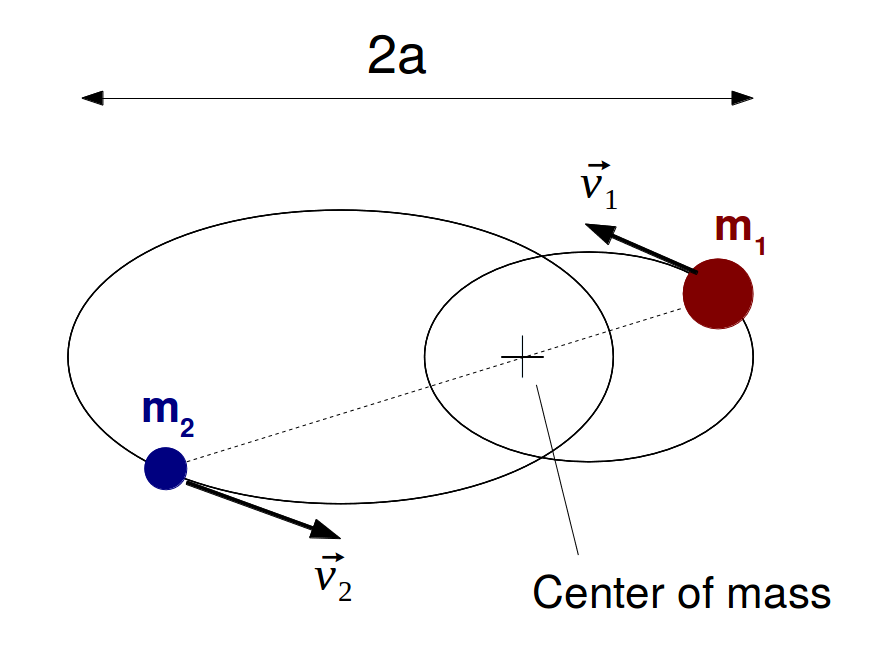
\includegraphics[width=0.93\textwidth]{Figures/0_elliptictrajectories.png}
        \caption{Schematic of a two-body system}
        \label{Fig:0_binary_2}
    \end{subfigure}
\caption{(a) Hubble observation of the binary star Albireo, fifth brightest star in the Cygnus constellation. Albireo A, the red star, is a close binary system itself (not represented on (b) for simplicity). The pair has a period of 213 years and a semi-major axis $a \simeq 66$ AU. }
\label{Fig:0_binary}
\end{figure}





The total energy of the binary can be expressed as a function of $a$ and $m_t$:

\begin{equation}
E = - \frac{G m_1 m_2}{2a} 
\end{equation}

\subsection{Why binaries ?}

Binary stars are extremely important for a variety of reasons. They can be a reservoir of energy, supporting the core of a cluster against collapse by giving away their internal energy to perturbers, effectively ejecting stars and heating the system, affecting its global evolution and stopping core collapse (e.g \citealt{Heggie1992}).

The statistical properties of binary star populations in dense stellar associations in particular may shed light on the discovery of multiple star-formation episodes in rich stellar clusters \citep{anderson2009}. For instance, binary stars enhance strong dynamical interactions which in turn may speed-up evolution off the main sequence and so boost enrichment of the ISM through winds (e.g., \citealt{Tailo2015}). Tight binaries of short-lived massive stars may evolve to produce exotic stellar remnants including black hole progenitors \citep{bacon1996,davies2009}. Blue stragglers, abnormally hot stars for the age of their host clusters, are thought to form in binary mergers, making them a dynamical record of the past binary population and dynamical state of the cluster \citep{Knigge2009}.

Finally, accurate knowledge of binary populations in stellar clusters enable good estimation of their dynamical mass, as the integrated velocity dispersion is largely biased by the binaries internal motions, see \cite{Rubenstein1997}.

\subsection{Multiplicity fraction}

In a stellar population, some fraction of stars will be found in multiple systems: some  in binaries and some in higher order hierarchies. A hierarchical triple is a stable 3-body bound system, a binary of which one of the component is a binary itself. The same principle applies to quadruple, quintuple, etc. One of the brightest stars in the night sky, Castor, is a sextuple hierarchical system, with 6 stars in a stable system.

Counting binaries and multiples is not straightforward: do you count triples as two binaries or three stars in a multiple system ? In their SPH simulation paper, \cite{Goodwin2004a} discuss several ways to measure the degree of multiplicity among stars in a system, each of them quantifying different properties, such as companion probability, companion frequency or pairing factor. 

Let  S be the number of single stars, and B,T, and Q the number of binary-, triple-, and quadruple systems, respectively. The fraction of multiple stars bound in binaries, triples, .. to the total number of multiple plus single stars, is

\begin{equation}
\label{Eq:0_fm} 
f_m = \frac{B + T + Q}{S + B + T + Q}. 
\end{equation}

This last  measure is used in seminal observationnal papers \citep{DM91,Raghavan2010} and is our adopted choice. As pointed out by \cite{Hubber2005}, $f_m$ in Eq. (\ref{Eq:0_fm}) has several advantages: 1) it  may be  restricted to a given mass $m$, setting  $S_m$ the number of single stars, and $B_m,\, T_m,\, Q_m$  the multiple stars with a primary of that mass ;  2)  the multiplicity fraction is observationally robust: when a binary is being reclassified as a triple, or an even higher order multiple system, the fraction does not change. 
 These definitions may be extended to cover a mass range  in a coherent way, by substituting $m \rightarrow \langle m\rangle$, the mean value over the range. This is useful mostly when comparing  systems with different stellar mass functions. 


\subsection{Observed population}
\label{Sec:0_raghavan}

\begin{figure}
\center
    \centering
    \begin{subfigure}[b]{0.48\textwidth}
    	\centering
        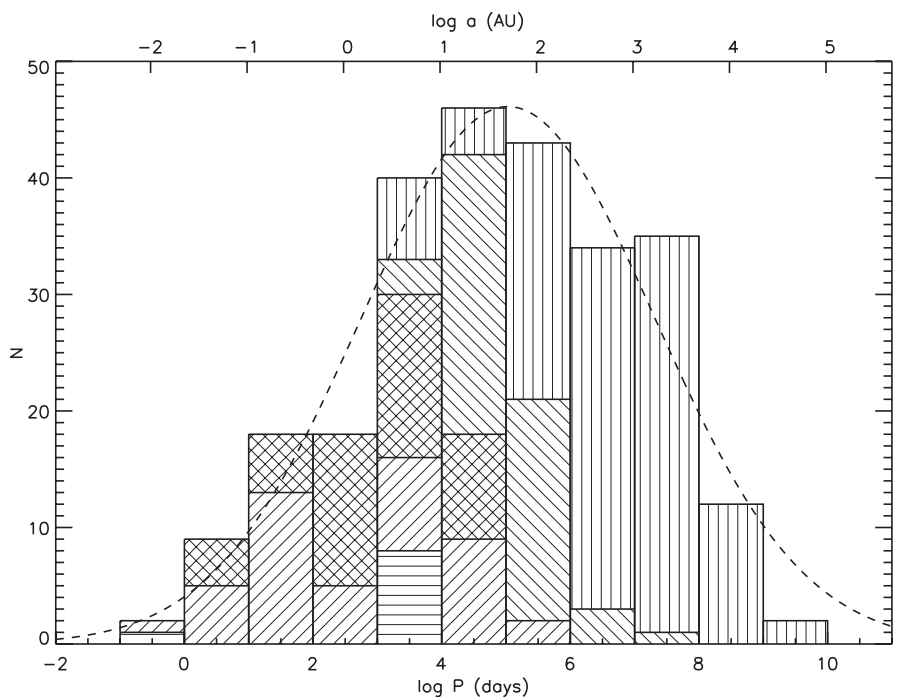
\includegraphics[width=\textwidth]{Figures/0_binperiods.png}
        \caption{Period and semi-major axis distribution}
        \label{Fig:0_binpop_1}
    \end{subfigure}
    ~~
    \begin{subfigure}[b]{0.48\textwidth}
    	\centering
        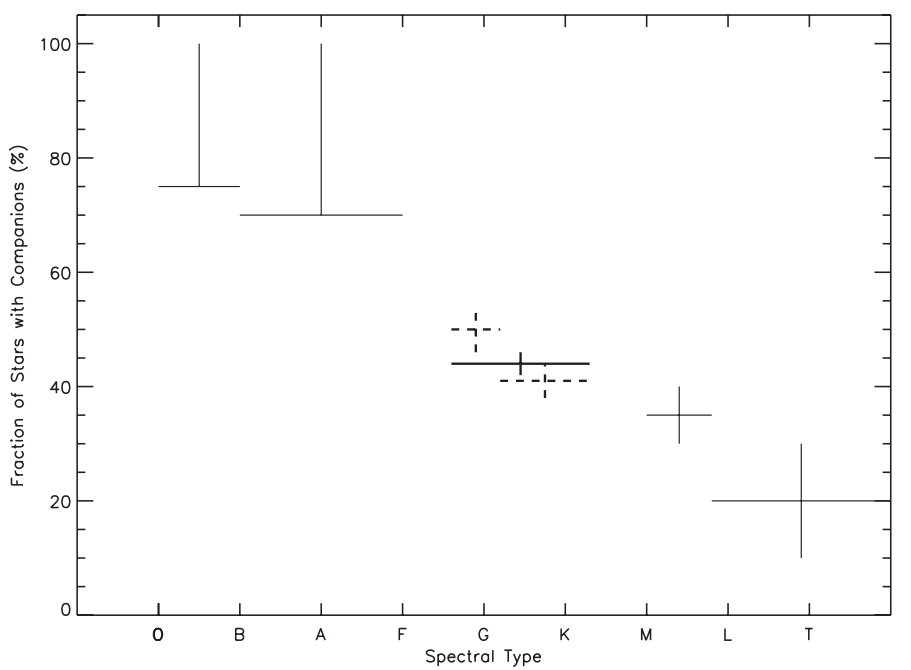
\includegraphics[width=0.97\textwidth]{Figures/0_binfraction.png}
        \caption{Binary fraction vs spectral type}
        \label{Fig:0_binpop_2}
    \end{subfigure}
\caption{(a) shows the observed distribution of period and semi-major axis observed in the field. Different hatchings show different observation techniques: horizontal lines show unobserved companions detected by the proper-motion acceleration of components, positively sloped lines show spectroscopic binaries, negatively sloped lines visual binaries, cross hatching show objects found with both, and vertical lines are objects with common proper motions. (b) was compiled from several surveys, detailed in Fig 4.? (to come later). Both figures were extracted from \cite{Raghavan2010}. }
\label{Fig:0_binpopulation}
\end{figure}




A seminal survey of binary solar-type stars in the field was performed by \cite{DM91}. This seminal paper was updated and completed by \cite{Raghavan2010}, who essentially confirmed the main results from the first study. They observed hundreds of F and G main-sequence stars in pairs and derived their binary parameters. The total binary fraction for these stars was found to be $\sim$ 53\% as binaries are quite common in any stellar population.
  The authors also derived a period distribution, extending from less than a day to more than a Myr. The distribution was consistently well fitted by a log-normal distribution. The period distribution for F and G stars (as well as K and M stars, see \citealt{Fischer1992}) is:
\begin{equation}
f( \log{P})\propto \exp \left[ \frac{- ( \log{P} - \mu_{logP})}{ 2 \sigma_{logP}^2} \right]
\end{equation}

with the peak value $\mu_{logP} = 5.03$, about 300 years, and the dispersion $\sigma_{logP} = 	2.28$, the distribution is shown on Fig~\ref{Fig:0_binpop_1}.

\cite{Raghavan2010} also compiled several observational studies of binaries with primaries of various spectral types. High mass stars, types O,B,A, (from 30+ down to 2$\Mo$) have a high multiplicity fraction, about 75\%  while lower mass stars such as M-dwarfs only have 10-30\% multiplicity, see Fig~\ref{Fig:0_binpop_2}. This trend of increasing multiplicity with increasing primary mass is found in many surveys.
Binary surveys are easier in the field due to the very large sample and low stellar density. To perform similar studies in young star clusters is much harder due to source crowding and embedded stars. \cite{Kouwenhoven2007} attempted to characterize the birth binary population in the OB association Scorpius OB2. They found a very high multiplicity fraction, consistent with 100\%, and a period distribution more consistent with a powerlaw than a log-normal distribution. From this survey and others, it is likely that the binary population in clusters undergoes an erosion through dynamical processing, with the field distribution as an end-result.

\subsection{Simulate binary populations in clusters}

As noted earlier, young clusters are born substructured, then undergo dynamical evolution. The rapid, global  merging of sub-structures would bring together stars at a different stage of their  formation (as in NGC1333, see \citealt{Foster2015}) while at the same time induce a shift from a clumpy Taurus-like profile to a more regular one. A simple but important question is how the internal dynamics of such complex configurations may affect the  characteristics of a population of binary stars. 

Many authors have explored this question through optimised initial conditions \citep{Kroupa2001,Marks2012} or fractal configurations evolved with N-body integrators \citep{Parker2011,Geller2013,Parker2014}. A common feature to all these studies is that the binary fraction drops over time regardless of their components (masses), due e.g. to close star-star encounters or heating from the external galactic tidal field, see Fig~\ref{Fig:0_binsim_1}. It was also shown that wide binaries are, as expected, more prone to destruction than more compact systems, as is illustrated by the evolution of the population seen in Fig~\ref{Fig:0_binsim_2}.

 \cite{Parker2014} pointed out that the distribution of semi-major axes $a$ of the field population is a strong function of the primary's mass: at fixed $a$, low-mass binaries carry less binding energy so the distribution cuts off at shorter separation ($\sim 20 $ AU) compared to that for binaries with a more massive primary ($\sim 300$ AU). Their study of fractal initial conditions show that gravitational dynamics enhances the dissolution of low-mass systems. This then provides a clue to account for the larger relative fraction of heavy stars in binaries, such as seen in a compilation by \cite{Raghavan2010}. 
 
 
\begin{figure}
\center
    \centering
    \begin{subfigure}[b]{0.48\textwidth}
    	\centering
        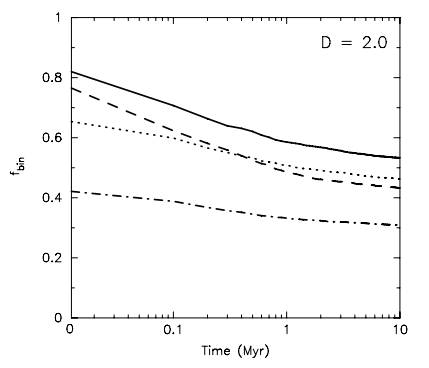
\includegraphics[width=\textwidth]{Figures/0_binfraction_evolution.png}
        \caption{Evolution of total binary fraction}
        \label{Fig:0_binsim_1}
    \end{subfigure}
    ~~
    \begin{subfigure}[b]{0.48\textwidth}
    	\centering
        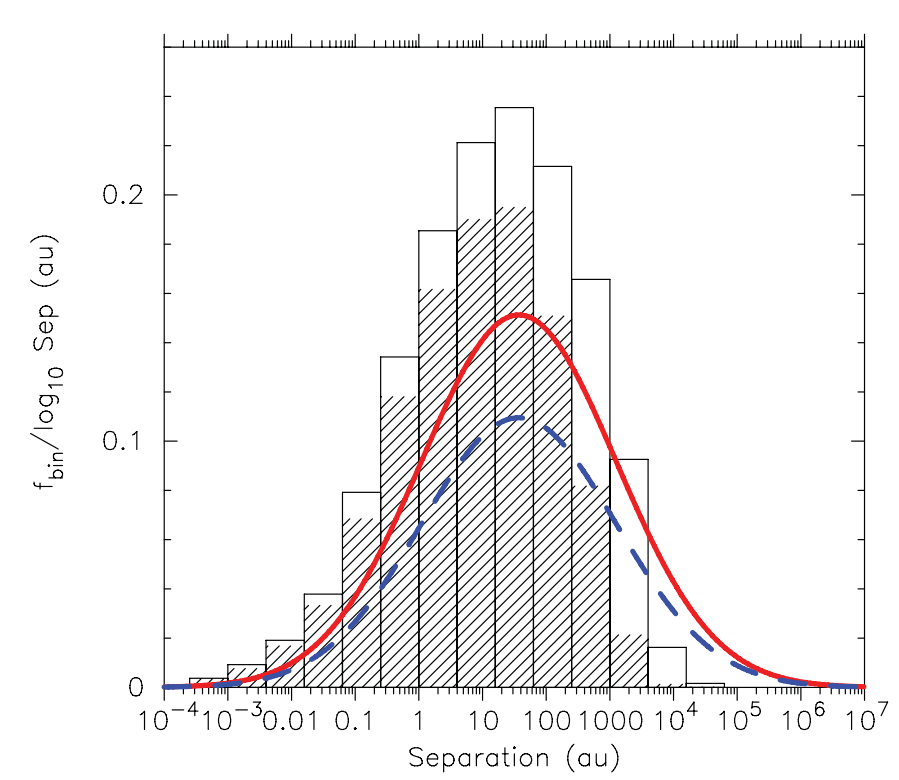
\includegraphics[width=0.97\textwidth]{Figures/0_separation_evolution.png}
        \caption{Evolution of semi-major axis distribution}
        \label{Fig:0_binsim_2}
    \end{subfigure}
\caption{(a): total binary fraction over time in a subvirial fractal system. Corresponding models for the solid, dashed, dot-dashed and dotted are respectively 100\% initial binary fraction with log-normal distribution, 100\% fraction with Kroupa distribution, field-like fraction with log-normal distribution and field and 75\% fraction with log-normal distribution. (b): 100\% initial binary fraction with an initial log-normal distribution (open histogram) and the evolved distribution after 1Myr (hashed histogram). Solid red and dashed blue lines are fits for, respectively, the G-dwarf and M-dwarf populations. Both figures were extracted from \cite{Parker2011}.}
\label{Fig:0_binsimulation}
\end{figure}

 
 
  We note that hydrodynamical calculations of star formation have found young heavy stars to be preferentially found in dense clumps \citep{Maschberger2010}. Furthermore, it is not clear yet whether binary populations should be tailored according to the total system mass because of the limited range of $M \sim 10^2$ to $ \sim 10^3 M_\odot$ of these studies \citep{Kroupa2001,Parker2011,Parker2014}. Recall that the intensity of the tidal field is a prime agent of binary heating.  A trend with mass may be expected on the ground that the drive to equilibrium of more massive systems leads to deeper potential wells (e.g. \citealt{Aarseth1988,Boily2002}). A steep potential will give rise to strong tidal fields which may disrupt bound sub-systems \citep{Boily2004,Renaud2011}. A definitive assesment of this effect is difficult to reach because the results are a strong function of the system initial mass distribution and kinetic energy content \citep{Boily2002,Caputo2014}.